\documentclass[floatfix, 12pt, apj]{emulateapj}

% latex ms.tex; bibtex ms; latex ms; latex ms; dvips ms; ps2pdf ms.ps ; gv ms.pdf
% latex ms.tex; bibtex ms; latex ms; latex ms; dvips ms; ps2pdf ms.ps ; open ms.pdf
% latex ms.tex; dvips ms; ps2pdf ms.ps ; open ms.pdf
\usepackage[paperwidth=8.5in, paperheight=11in, centering, margin=1in]{geometry}
\usepackage{amsmath}
\usepackage{epsfig}

\def\aap{{\it Astr.~Ap.}}     %Astronomy & Astrophysics%
\def\aaps{{\it A\&AS}}
\def\apj{{\it ApJ}}

\begin{document}
\title{Regularization Techniques for PSF--Matching Kernels. II. Pre--Filtering of Input Images}

\author{
A.C.~Becker\altaffilmark{1},
R.H.~Lupton\altaffilmark{2},
K.S.~Krughoff\altaffilmark{1},
et al.
}
\altaffiltext{1}{Astronomy Department, University of Washington, Seattle, WA 98195}
\altaffiltext{2}{Department of Astrophysical Sciences, Princeton University, Princeton, NJ 08544}

\date{\today}

\begin{abstract}

We describe a novel technique for reducing the numbers of false detections in difference images due to deconvolution (or sharpening) by the profile--matching kernel.
To accomplish this, we pre--smooth the input science image by its own point spread function (PSF) before performing profile--matching.
This results in a maximum--likelihood image for point source detection, which has a $\sqrt{2}$ broader point--source profile than the image PSF.
We then match a reference image to this smoothed image, effectively resulting in a point--source maximum likelihood difference image.
%The process of detection and measurement happens directly on this difference image.
By smoothing the input image, we reduce the number of conditions under which the reference image has to be sharpened to match the input image, which is a significant source of systematic false detections.
We compared this pre--filtering technique with the traditional (post--filtering) image subtraction approach using a suite of high--fidelity simulated images from the Large Synoptic Survey Telescope (LSST) phoSim effort.
We used a configuration environment to tune each pipeline, using an objective function that minimizes the mean--square residuals in a control sample of sources in the images.
We then ran a suite of images through image subtraction and source detection and measurement, using a simulated deep template image and three simulated science images that differ primarily in seeing.
Situations that lead to a deconvolution of the template image are shown to have a lower sensitivity to true variability, and higher incidence of false detections, due to enhancement of the image noise.
In this regard, using the pre--filtering technique is clearly preferred.
Under smoothing of the template image, we find that the quality of the difference image pixels is very similar under the two approaches.
However, the propagated per--pixel variance varies significantly at the detection stage, leading to differences in the rate of false detections.
We find a single--parameter correction to the effective detection threshold that brings the run of false detections with detection threshold in--line with theoretical expectations.
We examined several sources for this discrepancy.
An over or under--estimate of the background is shown to bias the ratio of positive--going to negative--going false detections, but does not significantly effect the total numbers.
However, a misunderstanding of the image noise is shown to significantly impact the overall false detection rate.
We find that even a 2\% misestimate of the noise may change the false detection rate by a factor of 1.5--2 at the 5--sigma detection threshold.
Under both pipelines, the propagated variance in the resulting difference images is within 1\% of the empirical variance.
However, with when post--filtering the difference images for detection, the variance is underestimated by 4--5\% (when not deconvolving), leading to an increase in the rate of false detections.
This suggests that the multiple integral transforms being applied to images lead to significant misestimation of the variance, as the pixels become correlated and current algorithms do not track the pixel covariance during these operations.
Finally, we note that in order for there to be less than 1 statistical false detection per LSST difference image, the detection pipeline must operate at a threshold of 5.5--sigma under median (0.6'') seeing conditions.

\end{abstract}
\keywords{methods: data analysis, techniques: image processing}

\section{Introduction}

{\bf TODO}

Image subtraction as a solution to general crowded--field variability detection.

PSF-matching as a means to image subtraction.

Sources of false detections (in binary classification these would be naturally referred to as ``false positives''.  However, since ``positive'' also may refer to the polarity of a difference image detection, and we indeed accept both positive--going and negative--going detections as ``false positives'', we choose to use the term ``false detections'' here to refer to these sources).

Machine learning as a way to address false positive rate.

LSST.

Alert stream.

Mention that one paper that talks about pre--filtering but not for this reason.

\section{PSF--Matching Algorithm}

Image subtraction proceeds by assuming that science image $S(x,y)$ can be modeled as a convolution of a reference template image $T(x,y)$ by a PSF--matching kernel $K(u,v;x,y)$ (indices $u,v$ indicate that the kernel itself is a 2--dimensional function, which varies as a function of position $x,y$ in the image.
During convolution and correlation there is an implicit summation over $u,v$).
The two images will have different point--spread--functions (PSFs), which are the time--averaged transfer functions of a point source through the Earth's atmosphere, telescope optics, and into the silicon of the detector before being read out.
The essence of image subtraction is to match the PSFs of these two images using a $K(u,v;x,y)$ so that they may be subtracted pixel by pixel.

In practice, it is assumed that the PSF--matching kernel may be decomposed using a set of basis functions $K(u,v) = \sum_i a_i K_i(u,v)$, where the coefficients in front of each basis are determined through:
\begin{eqnarray}
\label{eq-soln}
C_i & \equiv & (K_i \otimes T) \\ 
b_{i}  & = & \sum_{x,y} {{C_i(x,y) S(x,y)}\over{\sigma^2(x,y)}}   \nonumber \\
M_{ij} & = & \sum_{x,y} {{C_i(x,y) C_j(x,y)}\over{\sigma^2(x,y)}}  \nonumber \\
b_{i}  & = & M_{ij} a_{j}. \nonumber
\end{eqnarray}
In these equations, the terms $C_i$ come from a convolution of the template image with each basis function, and $\sigma^2(x,y)$ are the per--pixel variances.
The solution for $K(u,v)$ is determined by solving for each coefficient $a_i$, which represent the relative weights of each basis.

Point--spread--functions typically have spatial variation across an image due to high--order optical distortions and structure in the perturbing atmosphere; hence the PSF--matching kernel must also vary spatially.
To generate this model, it is assumed that the weights of the basis functions $a_i$ themselves vary spatially, i.e. $K(u,v;x,y) = \sum_i a_i(x,y) K_i(u,v)$.
In general, there is also a differential background map between the two images $b(x,y)$ that may be fit for using a low--order polynomial.
The final image difference is then calculated through $D(x,y) = S(x,y) - T(x,y) \otimes K(u,v;x,y) - b(x,y)$.

It is important to note that the choice of basis functions $K_i(u,v)$ is a degree of freedom in this problem.
Many implementations \citep{Alard98,Alard00} use a set of 3 Gaussians, each with a different width $\sigma_n$, and each modified by a Laguerre polynomial to a given order.
Subsequent studies \citep[e.g.][]{2007AN....328...16I} have suggested that a constant ratio be maintained between the different Gaussian widths, such that $\sigma_{n+1} = \beta \times \sigma_{n}$.
We adopted the value $\beta = 2.0$ for this work.
We set the overall scale for these widths by noting that, under the assumption that the PSFs of the images are themselves Gaussian ($\sigma_S$ for the science image and $\sigma_T$ for the template image), the width of the matching kernel $\sigma_K$ should be simply $\sigma_K^2 = \sigma_S^2 - \sigma_T^2$.
We used this width for the central Gaussian in a 3--component basis, with the smaller and larger Gaussians a factor of $1/\beta$ and $\beta$ different, respectively.

Detection on a difference image occurs after correlation of $D(x,y)$ with the science image's PSF, yielding a detection image $D'(x,y) = D(x,y) \circ PSF_S(u,v;x,y)$, where the $\circ$ operator denotes correlation.
The values of the pixels in $D'(x,y)$ provide a maximum--likelihood estimate of there being a point source at that position.
Detection occurs by searching for single pixels in $D'(x,y)$ that are more than $N$ times the square root of the per--pixel background variance.
The value of $N$ defines the detection threshold, and is also a degree of freedom in the problem, chosen to minimize the number of statistical fluctuations while maximizing the sensitivity for true sources of variability.
Once sources are detected in image $D'(x,y)$, measurement proceeds on the associated pixels in $D(x,y)$.

In this work we investigated two orders of operations for the optimal point--source filtering by the PSF.
In the first method, which is the classical implementation of the technique, we create a difference image that is then post--filtered with the PSF for detection:
\begin{eqnarray}
D_{Post}(x,y) & = & S(x,y) - T(x,y) \otimes K_{Post}(u,v;x,y)  \nonumber \\
D'_{Post}(x,y) & = & D_{Post}(x,y) \circ PSF_S(u,v;x,y).  \nonumber
\end{eqnarray}
In the second method, which we refer to as pre--filtering, we match the template image to a PSF--filtered science image:
\begin{eqnarray}
D_{Pre}(x,y)  & = & S(x,y) \circ PSF_S(u,v;x,y) - \nonumber \\
             &   & T(x,y) \otimes K_{Pre}(u,v;x,y) \nonumber \\
D'_{Pre}(x,y) & = & D_{Pre}(x,y). \nonumber
\end{eqnarray}
In this case, both detection and measurement happen on the same image.
For model--based measurements, the model will have to be smoothed with the image PSF before being compared to the pixels.

We note that since convolution commutes, ideally $K_{Pre} = K_{Post} \circ PSF_S$.
However, by pre--filtering the image that we are matching the template to, we increase the effective point--source profile width by a factor of $\sqrt{2}$.
This allows for less frequent {\it deconvolution} of the template image, when $\sigma_T > \sigma_S$.
This is valuable for two reasons.
First, deconvolutions are known to yield significant systematic features in difference images, due to enhancement of high--frequency noise outside the band limit.
Second, this allows for a deeper template image to be built from more input data, since the restrictions on the resulting $\sigma_T$ are less stringent.

%We note that in the standard analysis, detection is run on $D'_{Post}$ and measurement on the associated pixels in $D_{Post}$.
%In pre--filtering, both detection and measurement are run on $D_{Pre}$.
%For model--based measurements, this does require a modification of the algorithms to deal with the smoothing of the signal.

\section{Input Data}

In order to test the efficacy of these two approaches, we generated simulated images using the LSST PhoSim package v3.2.5 \citep{phosim}.
These images are high--fidelity simulations of the end--to--end LSST system, including effects from the atmosphere, optics, and detectors.
In order to establish an algorithmic baseline for the image subtraction code, we turned off certain confounding elements of the simulations, including airglow variations, cloud screens, tracking variations, quantum efficiency variations, diffraction, saturation, and blooming.
An input stellar catalog was generated to seed the simulations that included a random field with $\sim 1000$ stars for each 4000x4072 pixel LSST sensor, and a flat $r$-band magnitude range of $19<r<21$.
All stars in the sample had identical spectral energy distributions to avoid chromatic effects.
% km50_5000.fits_g20_5140.gz
For all sources, proper motion, parallax, and variability were set to zero.
Thus there is no intrinsic variability of any sort designed into the simulated images, and any detections in their differences will be by--definition false detections.

Four simulation runs were generated using the following configurations:
\begin{itemize}
\item {\tt Visit 0}: A 300s template image with an atmospheric seeing value of 0.88 arcsec.
\item {\tt Visit 1}: A 15s science image with 0.6 arcsec atmospheric seeing.
\item {\tt Visit 2}: A 15s science image with 0.88 arcsec atmospheric seeing.
\item {\tt Visit 3}: A 15s science image with 1.2 arcsec atmospheric seeing.
\end{itemize}
The seeing of the template image was designed to result in a sharpening deconvolution when compared to {\tt Visit 1}, and a smoothing convolution when compared to {\tt Visit 3}.
All observations were simulated at the zenith, and all images were simulated in the $i$--band.
Sky backgrounds in the resulting images were at the level of $\sim 150$ counts per pixel.
Nine sensors of the central LSST raft were simulated in each run, and the template visit PSF--matched and subtracted from each visit's CCDs, using both the post--filtering and pre--filtering pipeline.

A given image consists of three different layers, or planes, that track different bits of information.
The first plane contains the science pixels, which is the layer on which detection and measurement algorithms operate.
The second plane consists of a pixel--wise bitmask, indicating the quality of each pixel (was it saturated, or a detector defect) as well as detection information (was this pixel part of a source).
The third plane contains the pixel--wise variance, which is tracked through all additive, multiplicative, and integral transform operations.
The ``empirical'' variance of an image is estimated by taking all of the unmasked pixels and calculating their interquartile range, scaling by 0.741 (appropriate for a Gaussian distribution) and squaring the result.
The ``propagated'' variance of an image is estimated by taking all of the unmasked variance pixels, and calculating their mean or median.

\section{Optimizing the Algorithm}

We describe our image processing pipeline below, including the optimization of the image subtraction code using a control sample of sources.
This is followed by a discussion of the steps of point source detection and measurement in each pipeline.
For all pixel--level resampling operations, we chose to always operate on the template image given its larger signal--to--noise, and (in the case of real data) fewer artifacts such as dead pixels and cosmic rays.

\subsection{Pipeline Implementation}

At the start of processing, there are a pair of template and science images that are to be astrometrically and photometrically registered.
The process of astrometric registration refers to the exact alignment of the two images in pixel space, while photometric alignment refers to matching of the PSF shape, sky backgrounds, and zero--point.
From the input source catalog we choose 80\% of the stars to use in the registration process, with the remaining 20\% of the objects serving as a control sample to assess the effectiveness of $K(u,v;x,y)$ to subtract objects that were {\it not} used in the modeling process.
A direct image--to--image relative astrometric mapping was determined using the 80\% sample, and a sinc--based resampling kernel applied to the template image.
The resulting warped image was used as the image subtraction template $T(x,y)$.
The science image $S(x,y)$ and $T(x,y)$ were sent to the image subtraction task, whose purpose is to fit for $K(u,v;x,y)$ and to produce the difference image $D(x,y)$.

The first step in this process was to use the image PSF widths to define the {\it sizes} of the Gaussians' shapes in $K_i(u,v)$.
It is important to note that these widths are not fit parameters that are optimized under Equation~\ref{eq-soln}, and must be chosen by the user beforehand.
When $\sigma_S > \sigma_T$, a three--Gaussian basis was chosen, with the central Gaussian width being $\sqrt{\sigma_S^2 - \sigma_T^2}$, and smaller and larger Gaussians that were scaled in width by a factor of $\beta = 2$.
The degree of the modifying Laguerre polynomials were set using the mean--squared--error analysis below, with the smallest Gaussian typically modified by a degree 4--6 polynomial, and the larger Gaussians modified to lower order.
%We modified each of the Gaussians by a set of Laguerre polynomials of a given order.
%The smallest Gaussian was modified to the specified order, with the others modified by floor(order/2).
The total number of basis shapes in a given set is $\sum_{n=1}^{3} ({\rm degree}_n+1)\times({\rm degree}_n+2)/2$.

When $\sigma_T > \sigma_S$, we followed the prescription from \cite{0266-5611-26-8-085002} to choose basis widths, with the number of Gaussians fixed to three, and their Laguerre degree also fixed to three.
The widths of the Gaussians are determined through the algorithm specified in \cite{0266-5611-26-8-085002} Equation~40, using as inputs the sequence of Gaussians that we would have used to match a Gaussian of width $\sigma_S$ to $\sigma_T$ (i.e. as if we would have convolved the science image and not the template image).

The dimensions of the PSF matching kernel were chosen to be 6 times the largest Gaussian width, with a minimum kernel size of 21x21 pixels.
For kernels that are significantly smaller than this, the Gaussians have significant (non--zero) power at the kernel boundaries, leading to square systematic artifacts at the scale of the kernel in the difference images.

For each source indexed by $j$, we create substamps from each image $T_j(x,y)$ and $S_j(x,y)$ centered on that source.
These were used to fit for a local solution $K_j(u,v)$.
Note from Equation~\ref{eq-soln} that $C_i$, and thus the coefficients $a_i$, are derived from a convolution of the template substamps with the kernel basis function $K_i$.
This convolution means that pixels along the border of each substamp are rendered unusable, numbering half the kernel size around each edge.
To maintain a significant number of usable pixels for the computation of $C_i$, we set the stamp dimensions to be {\it twice} that of the kernel dimensions, such that the number of pixels remaining in $C_i$ after convolution is equal to the number of pixels in the kernel.

For each source, we solved for $K_j(u,v)$ to create a local difference image $D_j(x,y)$.
We evaluated several statistics on the pixels of this local difference image, which were normalized by the square root of the pixel variance to put the counts in units of standard deviations.
Under ideal conditions, this distribution should have a flat power spectral density.
We measured the mean sigma, the RMS of this distribution, the $\chi^2$ of these pixels normalized by the degrees of freedom (number of pixels in $D_j(x,y)$ minus the number of kernel bases), and the mean squared error.
These are referred to as the {\tt LOCAL} kernel metrics, and reflect how appropriate the chosen kernel basis is.

The ensemble of sources was then used to constrain a spatial model of the kernel $K(u,v;x,y)$.
For the spatial kernel model, we assumed that each of the kernel coefficients $a_i$ may be represented by a $N^{th}$ order 2--dimensional Chebyshev polynomial.
Having generated the full spatial solution $K(u,v;x,y) = \sum_i a_i(x,y) K_i(u,v)$, we evaluated the spatial kernel solution at the position of each source, created a new difference image using this kernel, and recalculated the metrics defined above.
These are referred to as the {\tt SPATIAL} kernel metrics.
Importantly, we also interpolated this solution to the positions of the control sample, which were explicitly {\it not} used in the spatial fit, and evaluated these same metrics.

The differences between the {\tt LOCAL} and {\tt SPATIAL} metrics for the training sample, as well as the values of the {\tt SPATIAL} metrics for the control sample, reflect the appropriateness of the spatial model and our ability to interpolate and extrapolate to the full extent of the images.
We used the mean square error (MSE) of the control sample to examine the tradeoff between bias and variance in the spatial interpolation.
We define the bias as $\left| data - model \right|$, the variance as $(data - model)^2$, with the MSE as {\tt bias$^2$ + variance}.  
In this context, the bias is the mean of the difference image, and the variance is the mean square of the difference image.
We found that N = 5 or 6 was sufficient to minimize the control sample MSE, or maximize the predictive power of the spatial model without overfitting.

Figure~\ref{fig:1} presents four sets of common image subtraction failure modes, and associated choices in pipeline configuration that may cause them.

\begin{figure*}[!ht]
  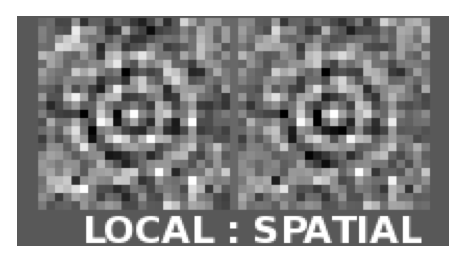
\includegraphics[width=0.5\textwidth, height=0.25\textwidth]{fig1a_crop.eps}
  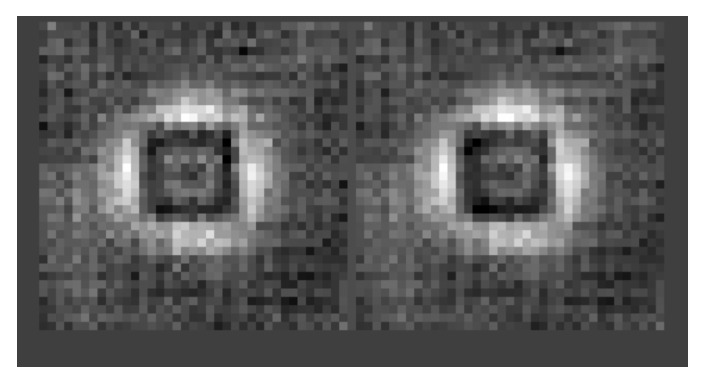
\includegraphics[width=0.5\textwidth, height=0.25\textwidth]{fig1b_crop.eps} \\
  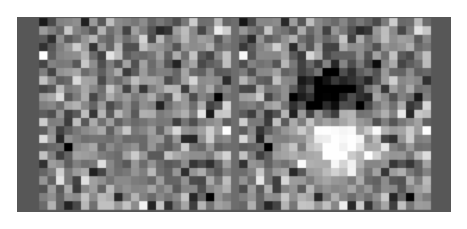
\includegraphics[width=0.5\textwidth, height=0.25\textwidth]{fig1c_crop.eps}
  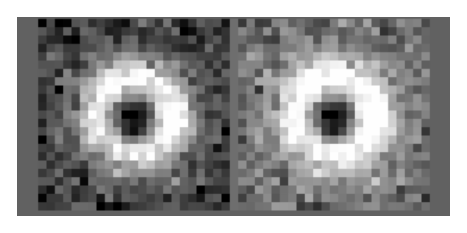
\includegraphics[width=0.5\textwidth, height=0.25\textwidth]{fig1d_crop.eps} \\
\caption{Four example panels showing failure modes of the image subtraction software.
  Each panel shows a pair of difference images; 
  in the {\it left} subpanel is the residual from the {\tt LOCAL} fitting, and in the {\it right} the residual from the {\tt SPATIAL} fitting.
  Starting in the upper left and proceeding clockwise, the first panel shows the residuals when deconvolving the template image; 
  the ringing in both solutions is characteristic of the deconvolution process.
  Upper right: a set of difference images where the kernel dimensions (kernel size) are too small given the widths of the Gaussians, such that the value of the kernel does not fall to zero along its boundary.
  This leaves square kernel--sized residuals around each object.
  Lower right: a set of images where the kernel shape (Gaussian sigma) is inappropriate to match the sources; 
  note that the {\tt LOCAL} residuals also show circular residuals, indicating the basis set itself is at fault (as opposed to the spatial model).
  Lower left: a set of images that demonstrate how the residuals degrade when the spatial kernel model is inappropriate.
  Note that the {\tt LOCAL} residuals appear to be white noise, while the {\tt SPATIAL} residuals show a clear dipole signature.
  For this reason, a comparison between the {\tt LOCAL} and {\tt SPATIAL} residuals is a useful diagnostic of the spatial model.
  The dipoles may also arise due to problems in the astrometric registration, or for individual extreme--color objects objects due to differential chromatic refraction.
}
\label{fig:1}
\end{figure*}


\subsection{Source Detection}

We next describe the process of source detection on the full difference images.
In post--filtering, we convolved the difference image with its PSF (by design, the same as the PSF of the science image) before detection.
In the case of pre--filtering, we detected on the difference image directly.
We looked for both positive and negative--polarity pixels more than $N$ sigma above the background, and performed the detection step at multiple significance thresholds to understand the numbers of false detections at each significance level.
These detections were merged together (e.g. to join the positive and negative lobes of a dipole) using a grow radius of 2 pixels.

%Since the fundamental image operations are the same, the images immediately preceding the detection step ($D'$) should have been {\it exactly} the same.
%As we will demonstrate in Section~\ref{sec-uh}, this was not exactly the case.

All difference image sources (henceforth diaSources) were associated with the reference catalog, with a matching radius of 3''.
We used this association to help assess if the diaSource was a source--associated false detection that came from the image subtraction software, or an orphan statistical fluctuation in the background.

%\subsection{Source Measurement}
%
%We outline the process of point--source PSF--weighted flux measurement below.
%We start with the definition of PSF--weighted flux:
%%
%\[F_j = \frac{\sum_{(x,y)}S_j(x,y) \times PSF_j(x,y)}{\sum_{(x,y)}PSF_j^2(x,y)}\]
%%
%where $S_j(x,y)$ is the image before PSF filtering, and $PSF_j(x,y)$ is an image of the PSF centered on the source.
%This equation assumes an isolated point source in a background--subtracted image.
%
%%We note that the convolution of an entire image $S(x,y)$ by its spatially varying $PSF(u,v;x,y)$, when evaluated at a single pixel, corresponds to multiplying the PSF matrix with a similarly sized matrix of pixels from the source image, centered on the source of interest.  
%The PSF--weighted flux in a post--filtered difference image $D$ is 
%%
%\[F_{Post,j} = \frac{\sum_{(x,y)}D_{Post}(x,y) \times PSF_j(x,y)}{\sum_{(x,y)}PSF_j^2(x,y)}\]
%while the flux in a pre--filtered difference image $D'$ is simply
%\[F_{Pre,j} = \frac{D_{Pre}(x,y)}{\sum_{(x,y)}PSF_j^2(x,y)}.\]
%
%To calculate the variance in the measurement, we assume a point source model for the intensity:
%%
%\[S(x,y) = A \times PSF(x,y) + \epsilon(x,y)\]
%\[\langle F \rangle = \langle \sum_{(x,y)} w(x,y)(A \times PSF(x,y) +\epsilon(x,y))\rangle\]
%%
%with a scaling factor $A$, white noise contribution $\epsilon(x,y)$, and
%%
%\[w(x,y) \equiv \frac{PSF(x,y)}{\sum_{(x,y)}PSF^2(x,y)}.\]
%%
%Since $\langle \epsilon(x,y) \rangle = 0$ and $\langle \epsilon(x,y) \times \epsilon(x',y') \rangle = \sigma^2(x,y)\delta(x-x', y-y')$:
%%
%\[\langle F \rangle = \sum_{(x,y)} w(x,y) \times A \times PSF(x,y)\]
%and
%\[\sigma^2_F \equiv \langle(F - \langle F \rangle)^2\rangle,\]
%such that
%\[\sigma^2_F = \frac{\sum_{(x,y)}PSF^2(x,y)\sigma^2(x,y)}{(\sum_{(x,y)} PSF^2(x,y))^2}.\]
%This implies that the error $\sigma_{F}$ on the flux at location x,y is a weighted sum of the per--pixel variance in the input image.
%
%%The center of each source is determined using an LSST adaptation of the SDSS centroiding algorithm \cite{photo}.
%%In general a source will not be centered on a pixel, so a Lanczos resampling kernel is used to shift the source to be centered on the nearest pixel before applying the measurement equations above.

\section{False Detection Rate}

To assess the ``quality'' of each implementation of the algorithm, we use as a metric the number of false positive--going and negative--going sources that are detected and measured in each difference image.
We discuss below our realized false detection rate, both in comparison to the theoretical statistical floor, and in intercomparison between the post and pre--filtering techniques.

\subsection{Theoretical \label{sec-analyticfp}}

To understand the nature of the base statistical false detection rate, we modeled source--free images (i.e.\ with a background described by a Gaussian process) using the statistics of Gaussian random fields \citep{Kaiser-PointSources}.
For an image with Gaussian noise convolved with a Gaussian PSF with width $\sigma_g$, the density of peaks above a given detection threshold $\nu$ is given by
\begin{equation}
n(>\nu) = \frac{1}{2^{5/2}\pi^{3/2}} \nu e^{-\nu^2 /2}.
\label{eq-theory}
\end{equation}
To estimate the number of random positive detections for a given image we must normalize this density by the total number of realizations of the PSF within the image, i.e.,
\begin{equation}
N_{total}(>\nu) = n(>\nu)*nrow*ncol/ \sigma_g^2
\label{eq-theorytot}
\end{equation}
where $nrow$ and $ncol$ are the number of image rows and columns.
In difference image analysis, we expect twice this number, since we are searching for both positive and negative--going fluctuations.

%To test our measurement suite, we created an empty sky--only simulated image, and recorded the number of detections in this image as a function of threshold.
%This showed good agreement with twice the amount indicated by Equation~\ref{eq-theorytot}, indicating that the simulated background is well described by a random Gaussian field.
Table~\ref{tab-fp} lists shows the theoretical number of false detections {\it per sensor} for an LSST--sized device, as a function of detection threshold.
We used a Monte Carlo approach to estimate the variance on the predicted false detection rate as a function of threshold, using $10^6$ realizations, to provide the uncertainties on the column values.
Note that to reduce the number of statistical false detections to less than 1 per sensor, under 0.6'' seeing conditions, the detection threshold should be set at a minimum of 5.5 sigma.
This value might indeed be allowed to float with seeing, such that the survey would make itself more sensitive to lower S/N objects under worse seeing conditions.

\begin{table*}[t]
\centering
\begin{tabular}{ccccc}
\hline
\multicolumn{5}{|c|}{Theoretical Number of False Detections per Sensor} \\
\hline
Visit    & FWHM (pixels) & $\sigma=4.5$ & $\sigma=5.0$ & $\sigma=5.5$\\
\hline
{\tt 1} & 3.0 & 114$\pm$11 & 12$\pm$3& 1$\pm$1\\
{\tt 2} & 4.4 & 54$\pm$8 & 5$\pm$2& 0.5$\pm$0.5\\
{\tt 3} & 6.0 & 29$\pm$6 & 3$\pm$2&0.2$\pm$0.4\\
\end{tabular}
\caption{{\rm Total number of false detections that we expect based on a 4000x4072 pixel sensor.
    This number is dependent on the seeing and detection threshold, so we list the values at a threshold of 4.5, 5.0, and 5.5 sigma for the seeings in the 3 visits used in this study.
    We list the total number of positive {\it plus} negative detections, which should be present in equal quantities.
    The variance is determined through Monte Carlo simulation.\label{tab-fp}}}
\end{table*}

\subsection{Empirical}

We next performed a detailed analysis of the false detection rate using our simulated image suite.
We report here the results for each of the 3 visits, and for pre-- and post--filtering for detection, using our optimal pipeline configurations.
We used measurement flags to remove spurious detections on the immediate border of the image; other than that we did no other cuts other than requiring that the centroid measurement was finite, which would be a realistic requirement for any real--time alert system reporting on these objects.
We separated the diaSources that match with the reference catalog (using a 3'' matching radius) from those that don't (referred to as ``orphans'') to investigate the origins of the detections.
We found no significant correlation of false detections rate with sensor within the raft; therefore we report the aggregate results for all 9 sensors in the analyses that follow.

\begin{table*}[t]
\centering
\begin{tabular}{clc|ccccc}
\hline
\multicolumn{8}{|c|}{False Detection Counts} \\
\hline
Visit   & Filtering & N$_{Expect}$ & N$_{Measured}$ &  N$_{Orphan}$ & N$_{Match}$ & N$_{Random}$ & N$_{-}$ / N$_{+}$\\
\hline
{\tt 1} & Pre      & 108$\pm$27   & 70      &60         & 10 & 3  & 1.8 \\ 
        & Post     & $\cdots$     & 143     &51         & 92 & 2  & 0.4 \\
{\tt 2} & Pre      & 45$\pm$18    & 42      &36         & 6  & 2  & 2.6 \\
        & Post     & $\cdots$     & 53      &45         & 8  & 2  & 0.5 \\
{\tt 3} & Pre      & 27$\pm$18    & 23      &23         & 0  & 1  & 2.8 \\
        & Post     & $\cdots$     & 36      &35         & 1  & 1  & 3.4 \\
\end{tabular}
\caption{{\rm Total number of diaSources detected at 5--sigma from all 9 sensors in raft 2,2 (N$_{Measured}$).
  N$_{Expect}$ lists the total number we expect to detect as random fluctuations, from Table~\ref{tab-fp}.
  Whether a detection is a match (N$_{Match}$) or an orphan (N$_{Orphan}$) is determined using a 3'' match radius with the input reference catalog.
  We list the number of background fluctuations that are expected to randomly associate with a Source N$_{Random}$, given the density of objects in the images and a 3'' match radius, assuming that N$_{Orphan}$ represents 96\% of the total population of detections from Gaussian fluctuations.
  \label{tab-bestfp10}}}
\end{table*}

The numbers N$_{Measured}$ of false detections in each case are given in Table~\ref{tab-bestfp10}, with the total number expected from the Monte Carlo analysis given as N$_{Expect}$.
We undertook a manual inspection of all difference images to associate the diaSources with sources in the images, ultimately using a 3'' association with the input source catalog to formally distinguish ``matches'' from ``orphans''.
Associations are listed in the N$_{Match}$ column of Table~\ref{tab-bestfp10}, with the unmatched false detections in the N$_{Orphan}$ column.
The former are likely to come from systematics in the subtractions of stars, while the latter would be due to fluctuations in the background.
We note two effects that impact N$_{Match}$.
The first is that, with a 3'' matching radius and our source densities, 4\% of random fluctuations will by--chance associate with a source.
Assuming that N$_{Orphan}$ represents 96\% of the background fluctuation population, we estimate the number of fluctuations from that same population that would have associated with sources as N$_{Random}$.
There is a slightly higher number of associations with sources than we would expect randomly (N$_{Match}$ $>$ N$_{Random}$), although this is rare and at the rate of 1 every 4--5 images.
In the last column of Table~\ref{tab-bestfp10} we list the ratio of negatively detected to positively detected diaSources.
The fact that these numbers are significantly different than 1.0 indicates that there are systematic issues in the reductions biasing the false detection population.

\section{Sources of False Detections}
We next examined in detail the nature of the false detections in these images.
This included an investigation of the sky subtraction in the images, how the image noise impacts the false detection rate, and the run of false detections with threshold.

\subsection{Sky Subtraction}

The ratio of negative to positive diaSources is significantly higher than 1.0 for all pre--filtering visits.
We examine modeling of the sky background as a potential source for this systematic.
The top panel of Figure~\ref{fig:2} shows contours of positive to negative false detections, overlayed on an over or under--subtraction vs. detection threshold plot.
We find that, at a 5--sigma detection treshold, a 1.5\% sky misestimate can bias the ratio of positive to negative sources by a factor of 2.
The bottom panel shows contours of the {\it total} numbers of false detections, positive plus negative, and we see that this value is relatively insensitive to the sky model.
As more detections of one polarity are found, fewer of the other are found, although the bias is to slowly increase the total numbers of false detections.
The observed negative--to--positive ratios of 2--3 suggest that there is a background oversubtraction of order $1-2\%$, causing low--sigma negative--going fluctuations to be measured at 5--sigma below the expected sky value of zero (Figure~\ref{fig:2}).
\begin{figure*}[!ht]
\centering
\centering{\includegraphics[width=1.0\textwidth]{fig2.eps}}
\caption{
Misestimation of the sky background value has an effect on both the number of false detections, and relative abundance of positive to negative false detections.
The top pane of this figure shows the relative number of +ve/-ve (-ve/+ve) detections if the sky background is under (over) subtracted at a particular fractional level.
The  bottom panel shows how the total number of false detections changes for the same misestimation.
This is not a strong function of the seeing; these numbers are appropriate for the 0.6'' simulation presented here.
}
\label{fig:2}
\end{figure*}

\subsection{Image Variance \label{sec-varmis}}

Figure \ref{fig:3} demonstrates the effect of misestimating the noise in the images for each of three different seeing values (0.6$^{\prime\prime}$, 0.88$^{\prime\prime}$, 1.2$^{\prime\prime}$ respectively).
In each case the top panel shows the number of additional expected false detections in an LSST--sized CCD, given a fractional misestimation of the noise in the image and a detection threshold.
A 1\% {\it under}--estimate of the noise corresponds to $\sim 4$ additional false detections at a threshold of $5\sigma$ in the best seeing case, compared to 12 expected (Table~\ref{tab-fp}), and 1 additional false positive in the worst seeing case, compared to 3 expected.
These additional numbers roughly double if the noise is underestimated by 2\%.
The bottom panels show the effect of {\it over}--estimating the noise in the measurement; as expected, the effect is to reduce the number of false detections.
A 1\% under-estimate of the noise typically results in 2 fewer false detections per chip, at 5--sigma.
\begin{figure*}[!ht]
  \includegraphics[width=0.33\textwidth]{fig3a.eps}
  \includegraphics[width=0.33\textwidth]{fig3b.eps}
  \includegraphics[width=0.33\textwidth]{fig3c.eps} \\
  \caption[]{ We plot here the expected change in the total number of false detections as a function of detection threshold and noise misestimate.
    The panels are for three values of image seeing, left--to--right 0.6'', 0.88'', and 1.2''.
    In each panel the top pane shows the rate increase when the noise is under--estimated, and the bottom shows the rate decrease when the noise is over--estimated.
    In all cases the counts are for the total number of false detections in a single 4000x4072--pixel random Gaussian field.
  }
  \label{fig:3}
\end{figure*} 

\subsubsection{Comparison of Empirical vs. Proposagated Noise Properties}


%{\bf good point: note that the curves nfp vs. threshold are
%  correlated, its a cumulative distribution}.

Since these images will have gone through multiple convolutions before reaching the detection stage, it is expected that the propagated per--pixel variance will not provide an exact representation of the empirical variance in the image planes \citep{Price-Stacking}.
Because the astrometric resampling uses a warping kernel that is designed to preserve the noise properties of the images, we expect that the kernel convolution will provide the largest source of such error.

To quantify this, we first compared the empirical variance in the image planes with the level tracked by the variance planes, for images $D$ and $D'$.
We calculated the ratio of the interquartile range of unmasked pixels in the image plane, multiplied by 0.741 and then squared, with the median of unmasked pixels from the variance plane.
The former represents the empirical variance, while the latter the propagated variance.
We investigate their ratio (empirical/propagated) at 2 stages in the processing: after creation of the difference image (image $D$), and immediately preceding detection (image $D'$; recall that for pre--filtering, $D = D'$).
These results are summarized in Table~\ref{tab-variance1}.
For pre--filtering, we find that the variance plane typically underestimates the true variance by $1\%$ for all visits.
When using post--filtering, the deconvolution {\tt Visit 1} yields a similar underestimate in the difference image, but for the other two visits the variance is tracked to better than 1\%, with a small RMS.
However, when post--filtering with the PSF, the variance becomes {\it overestimated} by nearly a factor of two for deconvolution {\tt Visit 1}, and {\it underestimated} by $4-5\%$ for the other visits.
This will yield a smaller number of statistical false detections during deconvolution, and a larger number of false detections during convolutions.
Looking at this in terms of sensitivity to true variability, this effect will lower the sensitivity to true transients during deconvolution, and heighten the sensitivity during convolutions.
The challenge in the latter case will be in distinguishing the true from systematic variability in the images.

\begin{table*}[t]
\centering
\begin{tabular}{clccc}
\hline
\multicolumn{4}{|c|}{Variance Ratios: Empirical / Propagated} \\
\hline
Visit    & $D_{pre} = D'_{pre}$ & $D_{post}$ & $D'_{post}$ \\
\hline
v6866601 &$1.012 \pm 0.002$&$1.018 \pm 0.005$&$0.599 \pm 0.017$ \\
v6866602 &$1.010 \pm 0.002$&$1.007 \pm 0.001$&$1.046 \pm 0.002$ \\
v6866603 &$1.015 \pm 0.003$&$1.008 \pm 0.001$&$1.045 \pm 0.003$ \\
\end{tabular}
\caption{{\rm Ratio of the empirical variance in the difference images, calculated using the square of (0.741 times the interquartile range), to the median of the variance plane.
  In all cases (except the deconvolution configuration) the variance plane represents an {\it underestimate} of the true variance in the images.
  We report the mean and RMS across all sensors.
\label{tab-variance1}}}
\end{table*}

\subsubsection{Investigating the Asymmetry Between Pre and Post--Filtering}

We next investigated the variance properties of the images that are input to the detection stage, i.e. the difference image itself in the case of pre--filtering, and the difference image convolved with its PSF in post--filtering.
In this comparison we look at the empirical variance of the pre--filtered image compared to that of the post--filtered image, and similarly compare the propogated variance.
These results are summarized in Table~\ref{tab-variance2}.
We find that the image pixels have very similar empirical noise properties at the detection stage, with the deconvolution visit having larger variance by $1\%$ but the other visits having essentially equal noise properties, with a bias towards the post--filtered data having slightly higher variance\footnote{For completeness, we note the median differences between the image planes at the time of detection are 3--4 counts (or 0.2 sigma relative to the empirical variance) for v6866601, 0.2 counts (0.02 sigma) for v6866602, and less than 0.1 counts (0.01 sigma) for v6866603.}.
The medians of the propogated variance pixels tell a different story.
For the deconvolution visit, the median per--pixel variance is $70\%$ higher in post--filtering.
This enhancement of the noise properties provides a clear preference for pre--filtering when post--filtering would result in deconvolution.
%While this will suppress the detections of false detections, it will also significantly suppress the detection efficiency for true variability.
For the other visits, the post--filtered per--pixel variance is relatively {\it lower} by $3-4\%$.
This will increase the sensitivity of the post--filtered data to false detections; as shown in Table~\ref{tab-bestfp10}, the rate is indeed larger using the post--filtering pipeline.
This analysis demonstrates that this is primarily due to an {\it underestimate} of the per--pixel variance in the post--filter processing: while the pre--filtered variance is a 1\% underestimate, the post--filtered variance is a 5\% underestimate.
As outlined by \cite{Price-Stacking}, this is likely due, at least in part, to a loss of pixel covariance when undergoing multiple convolutions, as covariance is not currently tracked in the LSST software used here.
In pre--filtering, the science image undergoes a single convolution, and the template image a pixel resamping and single convolution.
In post--filtering, the template image undergoes a pixel resampling and convolution, is subtracted from the science image, and then undergoes a second convolution with the PSF for detection.
As we have demonstrated here, this second convolution is where our variance bookkeeping lags the empirical variance.

\begin{table*}[t]
\centering
\begin{tabular}{ccc}
\hline
\multicolumn{3}{|c|}{Variance Ratios: $D'_{post} / D'_{pre}$} \\
\hline
Visit    & Empirical & Propagated \\
\hline
v6866601 & $1.011 \pm 0.016$    & $1.710 \pm 0.049$    \\
v6866602 & $1.001 \pm 0.001$    & $0.967 \pm 0.001$    \\
v6866603 & $1.002 \pm 0.001$    & $0.974 \pm 0.002$    \\
\end{tabular}
\caption{{\rm Ratios of the variance planes immediately before detection $D'$.
  Ratios are in the sense of the variance of the post--filtered image divided by the variance of the pre--filtered image.
  The first column represents the ratios of the empirical variance.
  The second column reports the ratios of the medians of the propagated variance planes.
  We report the mean and RMS across all sensors.
\label{tab-variance2}}}
\end{table*}


\subsection{Detection Threshold}
Obviously the number of false detections will be strongly dependent on the detection threshold.
In order to check the scaling of false detection rates with threshold, we ran the detection and measurement pipelines using several detection threshold values.
As discussed in Section~\ref{sec-analyticfp} one can predict the number of statistical false detections expected in a sensor at a given seeing and detection threshold.
The top row of Figure~\ref{fig:4} shows the results of this analysis.
From left to right the panels are for {\tt Visit 1} (0.6$^{\prime\prime}$ FWHM), {\tt Visit 2} (0.88$^{\prime\prime}$ FWHM) and {\tt Visit 3} (1.2$^{\prime\prime}$ FWHM) respectively.
We show the theoretical run of false detections vs. threshold in black, with a 1--sigma envelope coming from Monte Carlo simulations (Section~\ref{sec-analyticfp}).
The red squares show the empirical rates coming from the classical post--filtering analsis, while the blue circles are for the pre--filtering technique.
It is noteworthy that the deconvolution configuration shows an enhanced number of false detections at high significance.
Since our analysis shows that we should be {\it less} sensitive to statistical fluctuations under deconvolution, these should most prominently be coming from systematic mis--subtraction of source in the image.
These features typically appear as ringing in the images around bright sources, which trigger the detection algorithm.
As seen in Table~\ref{tab-bestfp10}, there are indeed an enhanced number of false detections that match to an image source (92 out of 143).
This demonstrates that the deconvolution process results in higher incidence of systematic features, and lower sensitivity to real fluctuations.

Also of note is that the majority of the curves lie {\it below} the theoretical expectations, although within the uncertainties.
This is not entirely unexpected, as each curve is strongly correlated, being a cumulative distribution, and represents only 9 samplings of the background random Gaussian field.
However, it may also signify a systemic issue in the analyses applied to these images.
Since our work here indicates that the total number of false detections are strongly sensitive to variance estimation, we explore a 1--parameter correction to the effective detection threshold to see if we can bring our data in--line with expectations.
Specifically, we define scaling factor $k$ to correct the counts at a given threshold:
\begin{equation}
n_{corrected}(>\nu) = n(> k * \nu)
\label{correction}
\end{equation}
and fit for $k$ {\bf HOW}.

The bottom panel of Figure~\ref{fig:4} shows the results of this correction, using $k = 0.975, 0.985 $~and~$ 0.99$ for {\tt Visit 1}, {\tt Visit 2}, and {\tt Visit 3}, respectively.
These results suggest our variance estimates are too {\it high}, and we are therefore detecting too {\it few} false detections.
{\bf This is consistent with the interpretation that the disagreement between the empirical variance of the image planes and propagated variance planes is due to missing information in the image planes.
That is, the ratio of empirical / propagated being larger than 1.0 is not because the propagate variance is too low, but that the empirical variance is too high.
That does not entirely make sense, because the pixels are correlated (smoothed).}
%This does not agree entirely with the analysis of the empirical variance, Section~\ref{sec-varmis} and Table~\ref{tab-variance1}, which suggest that our variance planes {\it underestimate} the true variance.
This makes clear that to operate near the theoretical floor in terms of false detection rate, it is imperative to track the variance in data at the 1\% level or better to optimize both the false detection rate, and the true detection efficiency.
\begin{figure*}[!ht]
  \centering
  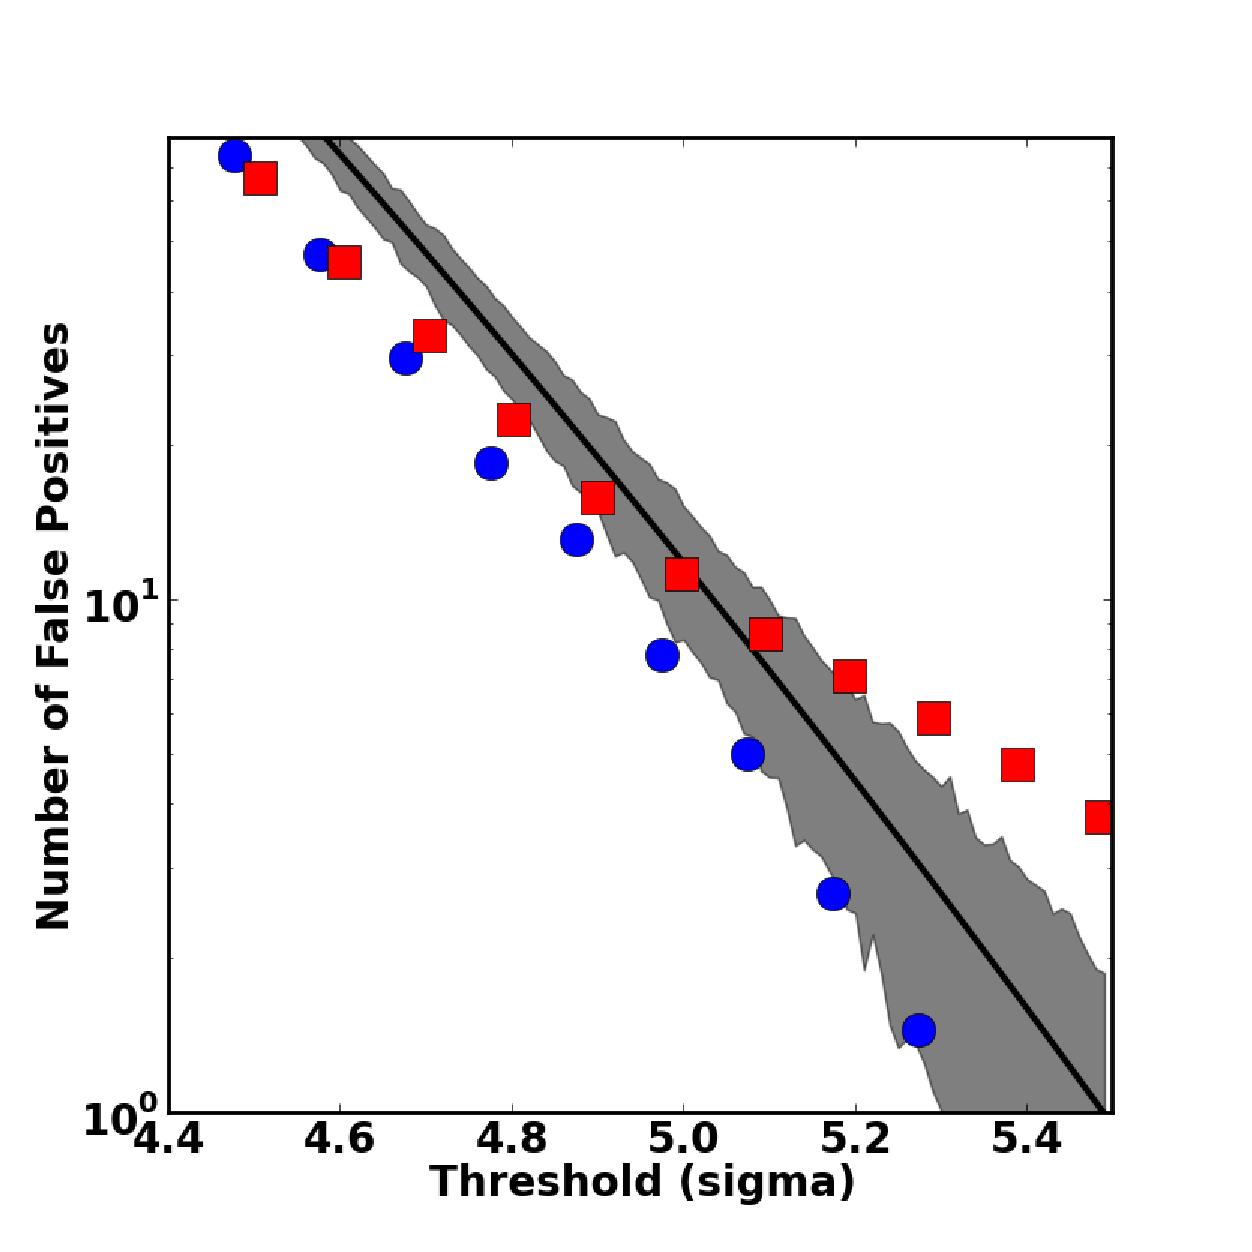
\includegraphics[width=0.32\textwidth]{fig4a.eps}
  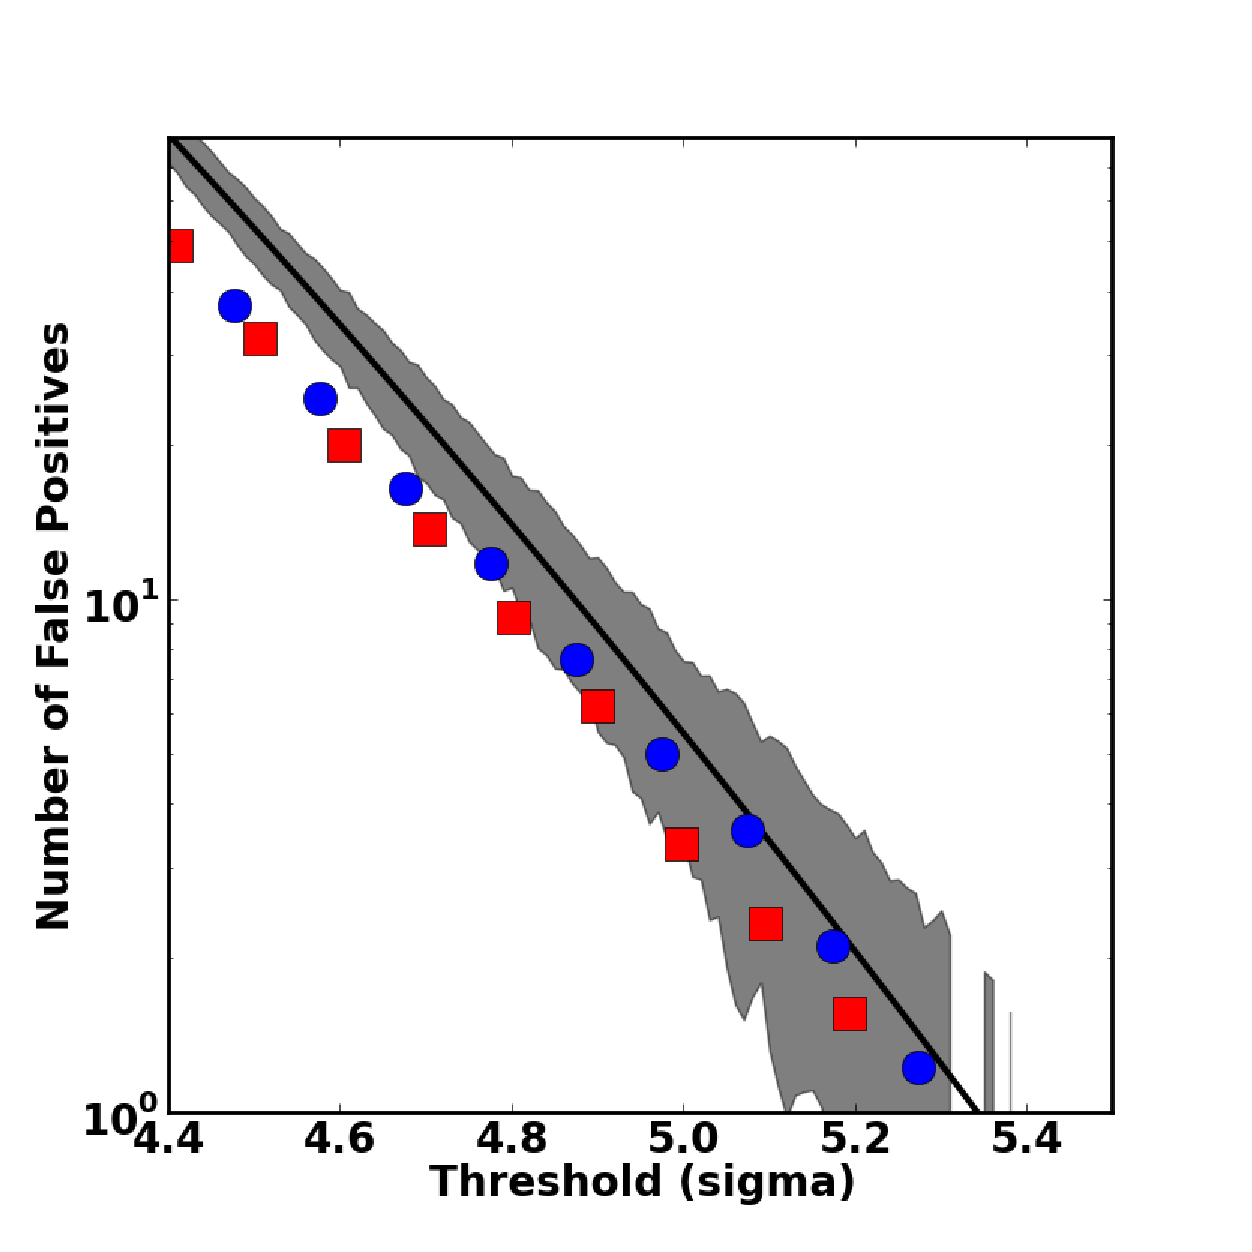
\includegraphics[width=0.32\textwidth]{fig4b.eps}
  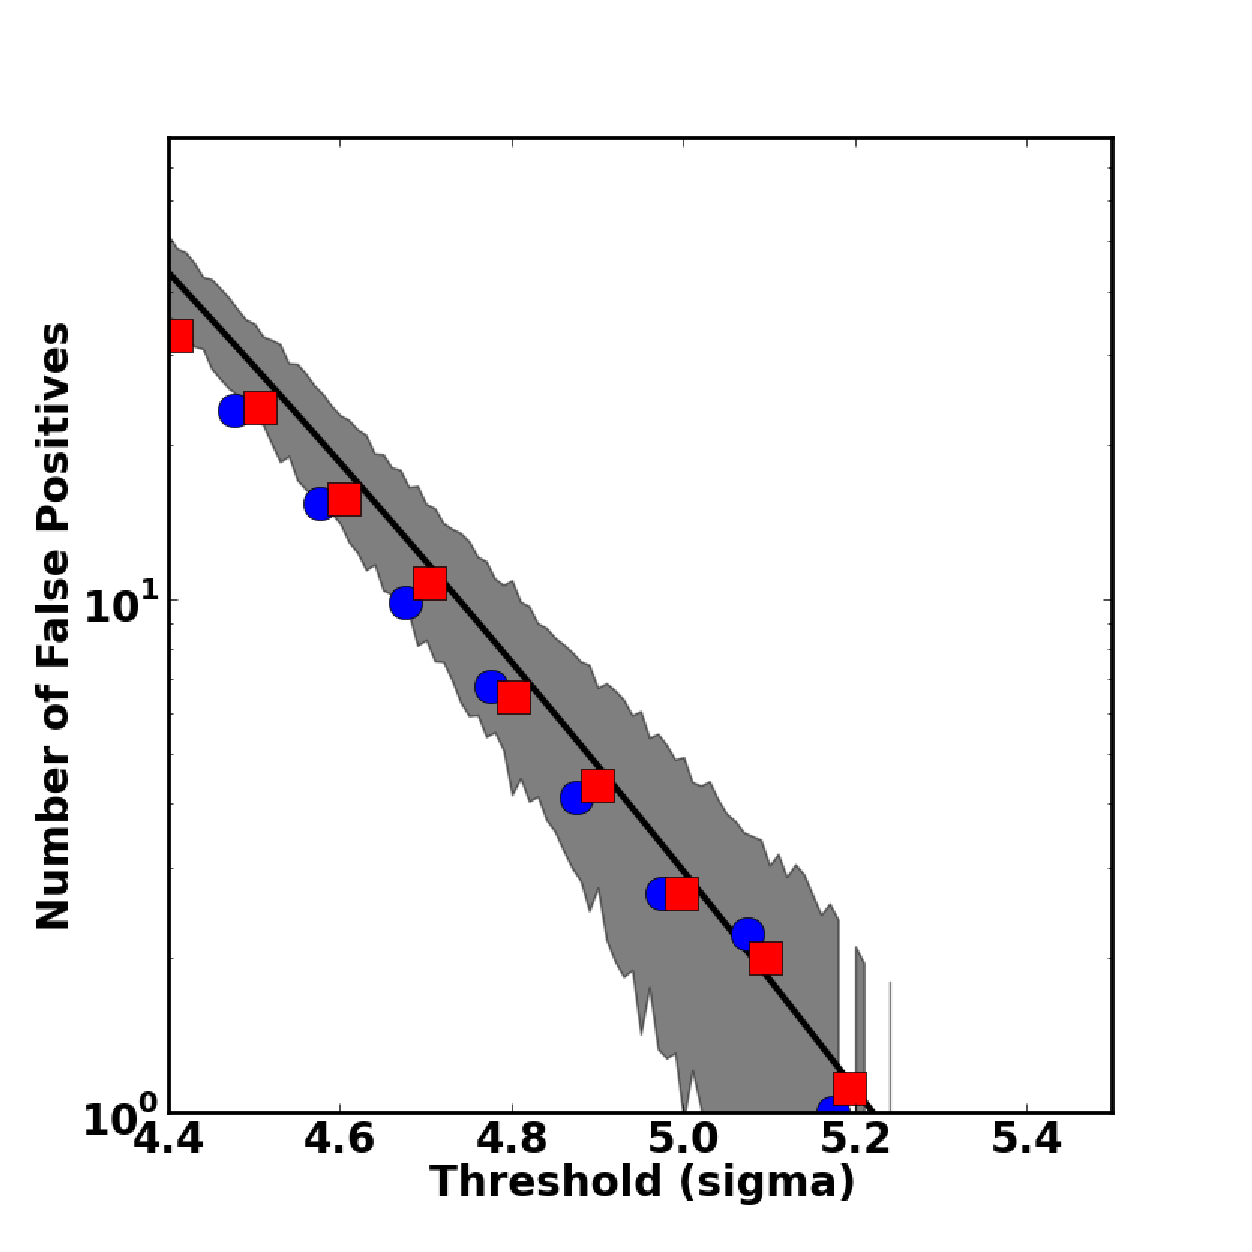
\includegraphics[width=0.32\textwidth]{fig4c.eps} \\
  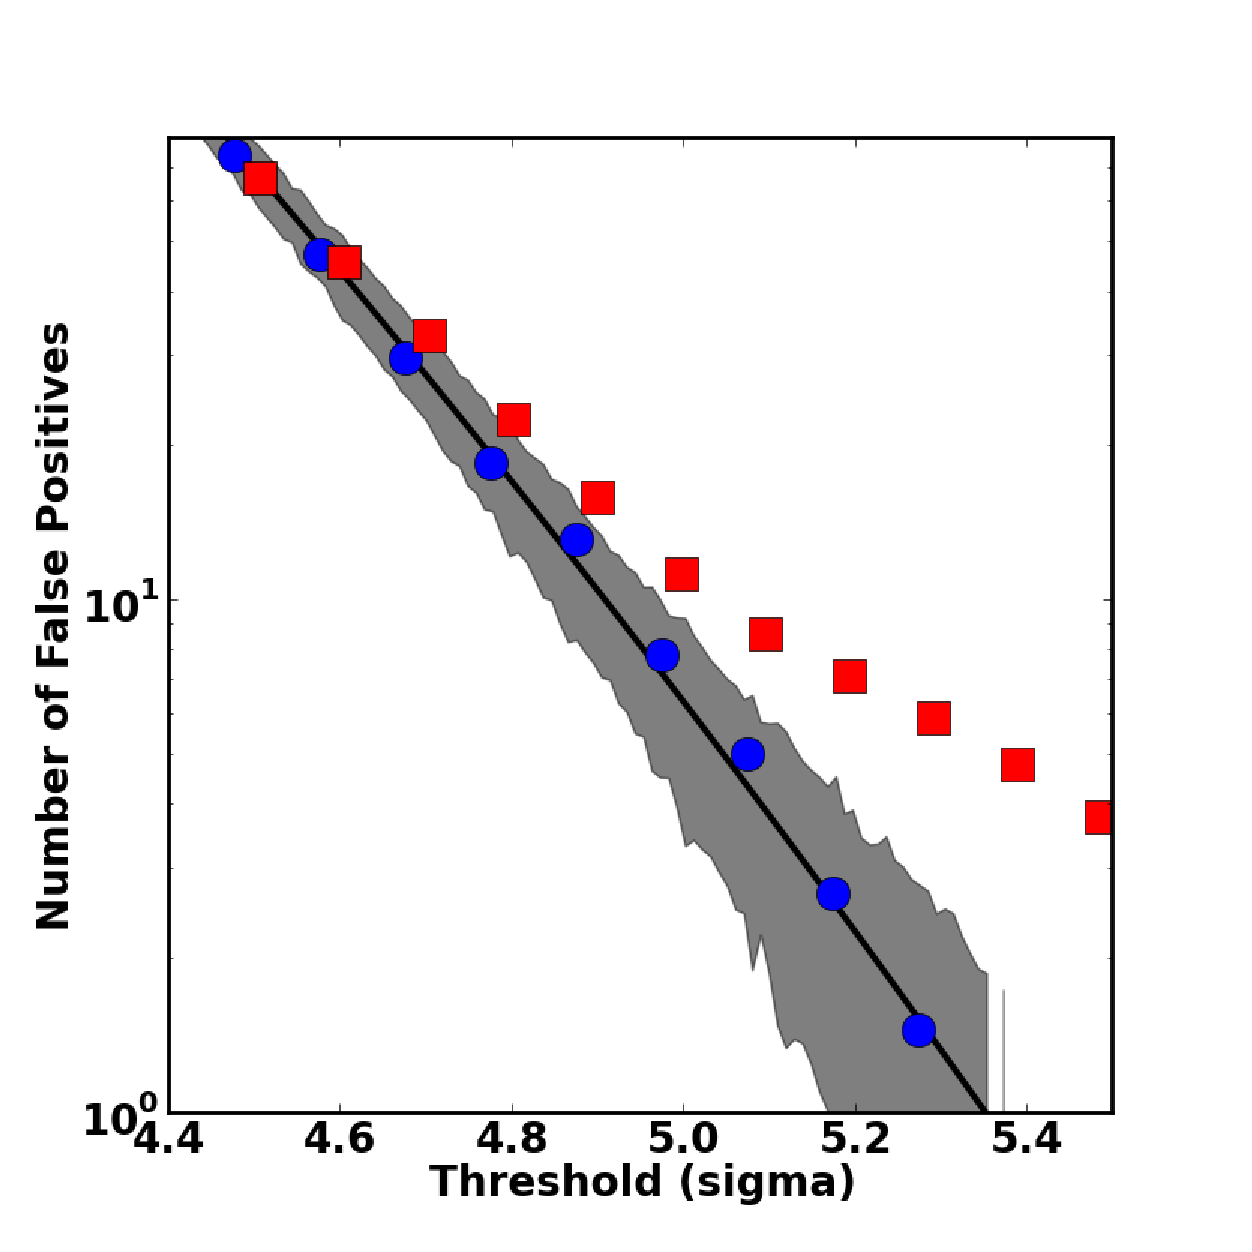
\includegraphics[width=0.32\textwidth]{fig4d.eps}
  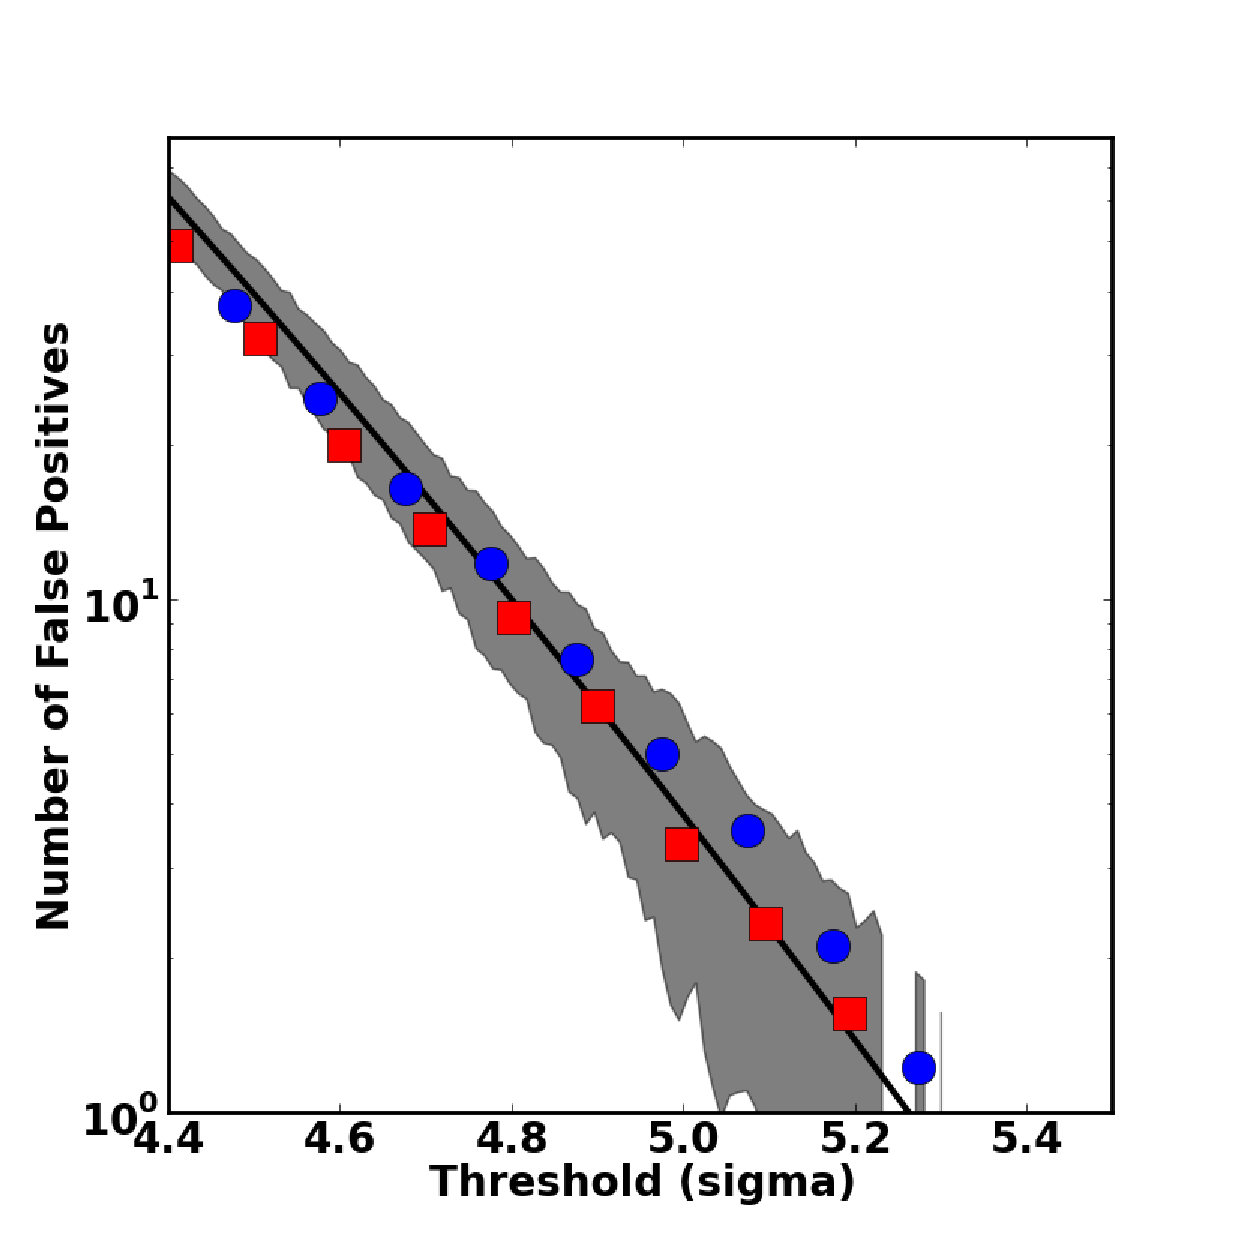
\includegraphics[width=0.32\textwidth]{fig4e.eps}
  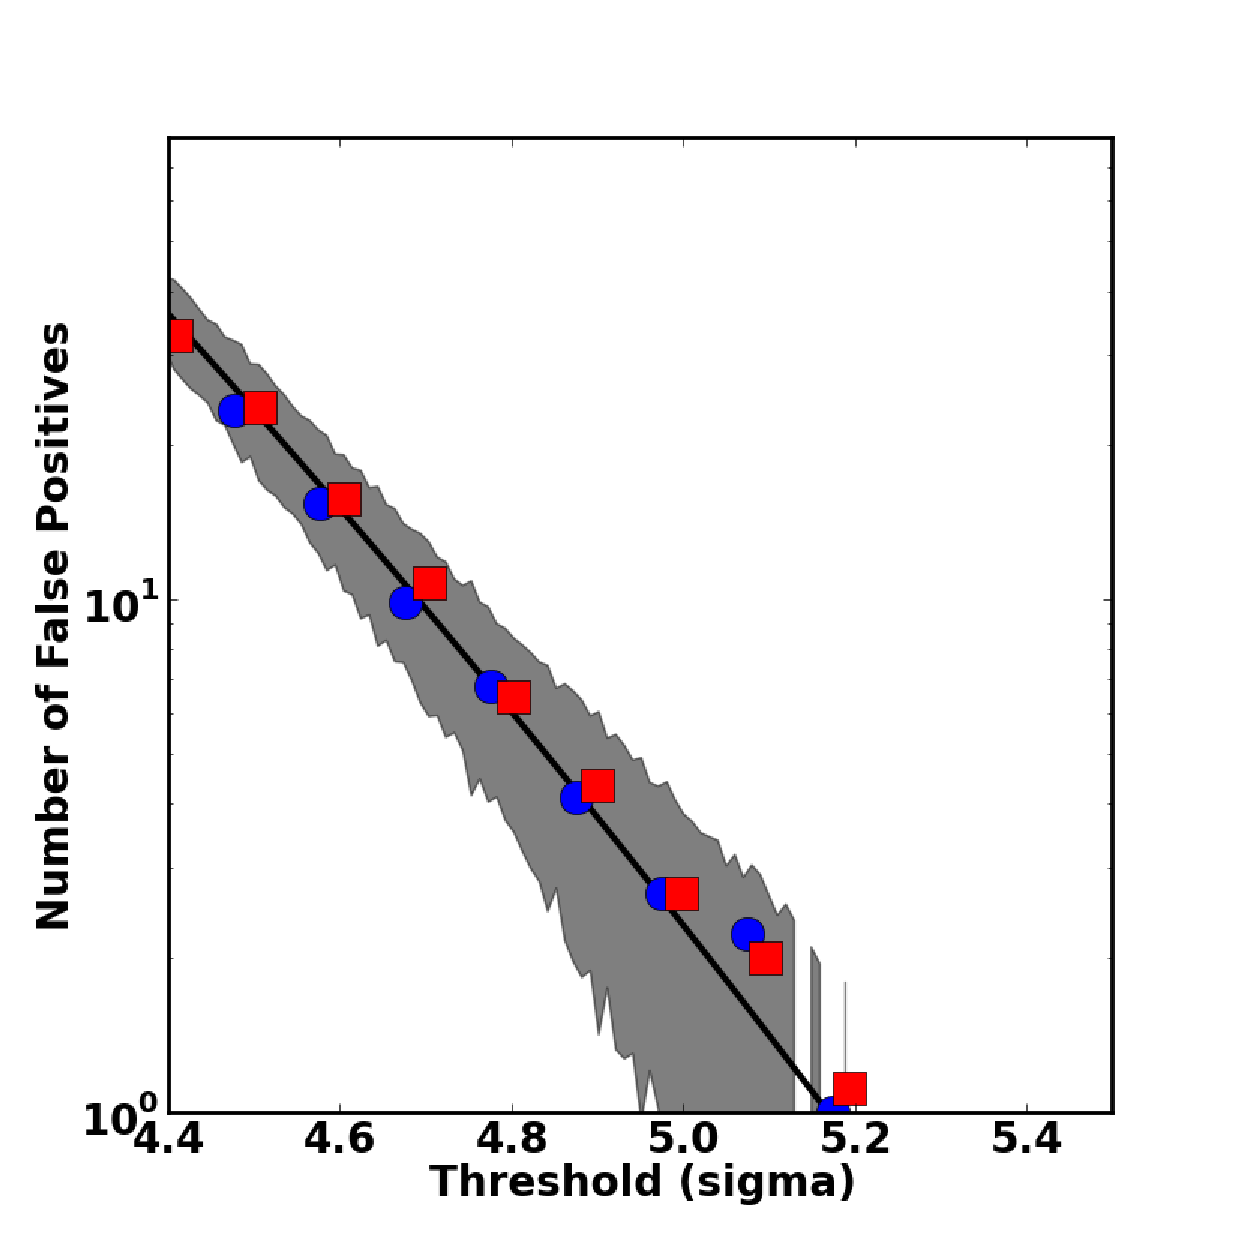
\includegraphics[width=0.32\textwidth]{fig4f.eps} \\
  \caption{Here we show the comparison of detected false positive count to the analytic prediction.
    In all cases the blue circles are the pre--filter case and the red squares are the post--filter case.
    In the bottom row we undertake a 1--parameter correction to align the predicted and measured values.
    The 2.5\%, 1.5\% and 1\% scaling in $k$ correspond to a 5\%, 3\%, 2\% over-estimation of the image variance, respectively from left to right in the bottom pane. 
    The shaded area is the 1-$\sigma$ confidence envelope determined from Monte Carlo simulations (Section~\ref{sec-analyticfp}).}
\label{fig:4}
\end{figure*}

\section{Discussion and Summary}

%We describe an end--to--end test suite to optimize the quality of a PSF--matching solution for image subtraction.
%The inputs are semi--idealized images that are science--grade simulations of Large Synoptic Survey Telescope data.
%This test suite is designed to optimize an objective function, which is the number of false positive--going and negative--going detections in the subtractions.
%We choose to use the predictive power of an out--of--sample test set to assess the overall quality of this PSF--matching solution.
%This test set is composed of point sources that were {\it not} used as part of the kernel solution; this solution is interpolated to their location using a spatial model.

%Within this test suite, we examine a new technique for pre--filtering the science images with their own point--spread--functions.

%The signal of a detection may also be misestimated by over or under subtracting the background.
%The result of errors in modeling the background is to change the ratio of positive to negative false detections.
%The top pane of Figure \ref{fig:2} shows how the ratio of sources of different polarities changes as a function of cutoff threshold.
%At a threshold of 5$\sigma$ one can observe 50\% more false detections of one polarity over the other with only a 1\% error in background modeling.
%Interestingly, the total number of false detections is not nearly as strong a function of background modeling errors.
%As the number of one polarity decreases, the number of the other polarity increases almost in proportion.
%This is shown in the bottom panel for Figure \ref{fig:2}.

In this analysis we examined several potential sources of false detections in subtracted images.
The first is due to misestimation of the variance in the images, which results in an enhanced (or deficient) rate of statistical fluctuations masquerading as variable sources.
Due to the steepness of the false detection rate with detection threshold, the variance in an image must be understood at the 1\% level or better to yield a clean set of diaSources.
The second is due to over or under--subtraction of the sky background, which will bias the ratio of positive to negative--going statistical fluctuations that are detected as sources.
However, the overall rate false detections has a shallow dependence on this function.
Since these two effects are somewhat orthogonal, the total numbers of orphan false detections (not associated with image sources) and the ratio of positive--going to negative--going orphans provides a joint constraint on the accuracy of the image variance calculations and of the background subtraction, respectively.
Finally, the process of deconvolution is shown to produce a decreased sensitivity to statistical fluctuations, due to enhancement of high frequency noise.
However, the artifacts of deconvolution around sources are themselves detected as an enhanced rate of systematic false detections, making this a worst--case treatment.

The pre--filtering of the science images by their PSF before template PSF--matching helps to avoid deconvolution except in the most extreme circumstances (when the FWHM of the template is $\sqrt{2}$ smaller than the science image).
In this regard, the process provides a clear advantage over the standard post--filtering technique.
In addition, the pre--filtering image variance in the source detection stage is consistently within 1\% of the empirical image noise, which is not the case for post--filtering.
However, a downside to this technique is that source measurement must also happen on this filtered image.
Because the image has been smoothed, higher order moments such as shapes will be smoothed.
Model--based shape measurements will have to themselves be smoothed by the PSF before comparing to the image pixels, necessitating a modified source measurement suite.
A potential but computationally expensive approach would be to create both pre--filtered and post--filtered difference images, and perform source detection on the pre--filtered image and source measurement on the post--filtered image.

We summarize the salient points of the analysis below:

\begin{itemize}

%%%

\item Our simulated image suite allows us to control the ground truth behind the images, which is invaluable in understanding the nature of false detections under image subtraction.

\item At the 5--sigma detection threshold, for the range of seeings considered in this study, the theoretical rate of false detections per LSST sensor numbers between 3--12, depending on seeing.
  This function is steep and seeing dependent; by increasing the detection threshold to 5.5 sigma this number may be lowered to less than 1 per sensor down to seeings of 0.6'' (Table~\ref{tab-fp}).
  This translates to of order 2 * $10^5$ per night for LSST, assuming 1000 visits / night.
  The steepness of the false detection function will enable control of the number of statistical false alerts by small modifications of the detection threshold.

\item Due to the steepness of this function, the number of false detections is strongly dependent on the variance being correct.
  When detecting at 5--sigma, having the noise underestimated by 2\% leads to an increase in statistical false detections by a factor of 1.5--2 (Figure~\ref{fig:3}).

\item When strongly deconvolving, the post--filtered variance is 70\% {\it higher} at the time of detection compared to the pre--filtered data (Table~\ref{tab-variance2}).
  This is consistent with the understanding that deconvolution increases high frequency noise in the images, and yields a {\it lowered} detection efficiency for true variability in deconvolved data.
  Systematic ringing features around sources also yield an enhanced rate of systematic false detections in deconvolved images.
  For this reason, pre--filtering is clearly preferred to post--filtering in the case of significant deconvolution.

%\item For non--deconvolved image subtraction, pre--filtering performs as well as post--filtering in terms of the number of false detections, when corrected for variance underestimate (Figure~\ref{fig:4}).

\item An empirical computation of the variance from the image plane, compared to the median propagated variance in the variance plane, indicates that the software consistently underestimate the variance in pre--filtering by $1-2\%$, and in post--filtering by $4-5\%$ (when not strongly deconvolving; Table~\ref{tab-variance1}).
  The post--filtering discrepancy is shown to arise from the PSF--filtering of the difference image immediately before detection.
  This is likely due, at least in part, to the double--convolution that is happening to the template image, and the lack of covariance tracking within the software.

\item The ratios of the empirical variance of the detection images between pre--filtering and post--filtering are similar to within $1\%$ (Table~\ref{tab-variance2}).
  However, the propagated variance in the post--filtered data is $3-4\%$ {\it lower} in the post--filtered data, leading to a larger number of false detections when using the variance plane as the definition of sigma (Table~\ref{tab-bestfp10}).


%%%

\item The post--filter pipeline can produce difference images with a minor deconvolution ({\tt visit 2}) at a quality commensurate with a subtraction that uses a smoothing convolution ({\tt visit 3}).

%%%

\item We find that the overall number of false detections is not strongly sensitive to bulk background misestimation (Figure~\ref{fig:2}).

\item However, the ratio of positive to negative--going false detections is strongly dependent on background fitting, with a 1\% error in the background causing 50\% more false detections of one polarity over another (Figure~\ref{fig:2}).

\item Our empirical negative to positive false detection ratio is 2--3 for pre--filtering, indicating a bias in the background levels of 1--2\%.
  Similar ratios are seen in post--filtering, although they vary from over-- to under--subtraction of the background (Table~\ref{tab-bestfp10}).

%%%

\item The measured false detection rate at 5--sigma is within the variance of the expected false detection rate arising from a random Gaussian field (Figure~\ref{fig:4}).

\item The measured false detection rate is seen to scale with detection threshold in a manner consistent with theory (Figure~\ref{fig:4}).
  A 1--parameter correction to the effective detection threshold by 1--2.5\% brings these relationships into almost exact correspondence.
  Accordingly, optimization of the false detection vs. true source detection efficiency will require an empirical understanding of the variance at the 1\% level.

\end{itemize}

\section*{Acknowledgments}
LSST blurb here.

\bibliographystyle{apj}
\bibliography{refs}

\end{document}
